\documentclass{beamer}
%AMDG
\usepackage{amsmath, amsthm, amssymb}
\usepackage{hyperref}
\usepackage[slovene]{babel}
\usepackage[utf8]{inputenc}
\usepackage[T1]{fontenc}
\usepackage{epigraph}
\usepackage{pdftexcmds}
\usepackage{fancyref, nameref}
\usepackage{epigraph}
\usepackage{cleveref}
\usepackage{verbatim}
%\usepackage{enumitem}
\usepackage{multicol}
\usepackage[nomessages]{fp}
\usepackage{fancyhdr}
\usepackage{multirow}
\usepackage{mathtools}
\usepackage{graphicx}
\graphicspath{ {img/} }



\usepackage{tikz}

\usetikzlibrary{ matrix,      % For easy node positioning
                 fit,         % For easily fitting nodes inside another one
                 positioning, % For easy node-relative placements
                 shapes, 	  % For elipse snd so
               }


\usetheme{Warsaw}

\newenvironment{remark}
{\textbf{Opomba:}}
{}

\uselanguage{Slovene}
\languagepath{Slovene}

\usetheme{Copenhagen}

\deftranslation[to=Slovene]{Theorem}{Izrek}
\deftranslation[to=Slovene]{Example}{Primer}
\deftranslation[to=Slovene]{Definition}{Definicija}

\newcommand{\subscript}[2]{$#1 _ #2$}

\newcommand{\twopartdef}[4]
{
	\left\{
		\begin{array}{ll}
			#1 & \mbox{; } #2 \\
			#3 & \mbox{; } #4
		\end{array}
	\right.
}


%operatorji
\newcommand{\ord}{\ensuremath{\operatorname{red}}} % red grupe/elementa
\newcommand{\Mod}[1]{ \ (\text{mod}\ #1)}

\beamertemplatenavigationsymbolsempty

\setbeamerfont{page number in head/foot}{size=\large}
\setbeamertemplate{footline}[frame number]

\usetheme{Antibes}

\author{Kralj Samo, Koprivec Filip}

\title{Mreže}
\institute{FMF}
\date{\today}

\begin{document}
\begin{frame}
	\titlepage
\end{frame}

\begin{frame}
	\tableofcontents
\end{frame}

\begin{frame}
\section{Osnovne definicije}
\subsection{Urejenost}
\frametitle{Urejenost}

\begin{definition}
Naj bo $\mathcal{L}$ množica, relacija $\leq$ je \textbf{(šibka) delna urejenost}, če je
\begin{itemize}
\item refleksivna ($a \leq a$)
\item antisimetrična ($a \leq b \land b \leq a \implies a = b$)
\item tranzitivna ($a \leq b \land b \leq c \implies a \leq c$)
\end{itemize}
\end{definition}

\begin{remark}
Občasno smo nekoliko "šlampasti" in za lažjo predstavljivost uporabimo tudi relacijo $\geq$, ki jo definiramo kot $a \geq b \iff b \leq a$
\end{remark}

\begin{block}{Dogovor}
Naj bo $\mathcal{L}$ množica urejena z relacijo delne urejenosti $\leq$ in $x,y \in \mathcal{L}$
\end{block}

\end{frame}

\begin{frame}
\subsection{Supremum in infimum}
\frametitle{Supremum in infimum}

\begin{definition}
$S$ je \textbf{supremum} $x$ in $y$, če velja: 
\begin{itemize}
\item $S \geq x \land S \geq y$ (Zgornja meja)
\item $\forall S' \in \mathcal{L} \implies (S' \geq x \land S' \geq y \implies S \leq S')$ (Je najmanjša zgornja meja)
\end{itemize}
označimo: $S = x \lor y$ 
\end{definition}

\pause
\begin{definition}
$s$ je \textbf{infimum} $x$ in $y$, če velja: 
\begin{itemize}
\item $s \leq x \land s \leq y$ (Spodnja meja)
\item $\forall s' \in \mathcal{L} \implies (s' \leq x \land s' \leq y \implies s' \leq s)$ (Je največja spodnja meja)
\end{itemize}
označimo: $s = x \land y$ 
\end{definition}

\end{frame}

\begin{frame}
\subsection{Definicija mreže}
\begin{definition}
Množica $\mathcal{L}$ je \textbf{linearno urejena}, če za poljubna $x,y$ velja $x \leq y$ ali  $y \leq x$ 
\end{definition}
\pause
\begin{definition}
Množica $\mathcal{L}$ je \textbf{mreža}, če ima poljuben par $x,y$ infimum in supremum.
\end{definition}

\end{frame}

\begin{frame}
\subsection{Osnovni primeri mrež}
\frametitle{Osnovni primeri mrež}
\begin{columns}

\begin{column}{2cm}
	\begin{center}
	$\mathbb{N}, \leq$
	\end{center}
  \begin{figure}
  \centering
  \begin{tikzpicture}[scale=1]
    \node (a) at (0,0) {};
    \node (c) at (0,-2) {$2$};
    \node (d) at (0,-3) {$1$};
    \node (e) at (0,-4) {$0$};
    \draw  (c) -- (d) -- (e);
    \draw[dotted] (c) -- (a);
  \end{tikzpicture}
  \end{figure}
\end{column}

\begin{column}{2cm}
  \begin{figure}
  \centering
  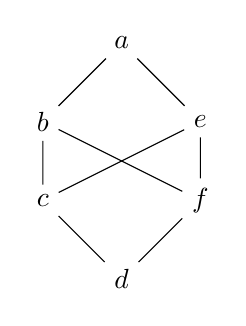
\begin{tikzpicture}[scale=1]
    \node (a) at (0,0) {$a$};
    \node (b) at (-1,-1) {$b$};
    \node (c) at (-1,-2) {$c$};
    \node (d) at (0,-3) {$d$};
    \node (e) at (1,-1) {$e$};
    \node (f) at (1,-2) {$f$};
    \draw (a) -- (b) -- (c) -- (d) -- (f) -- (e) -- (a);
    \draw (f) -- (b);
    \draw (c) -- (e);
  \end{tikzpicture}
  \end{figure}
\end{column}

\begin{column}{2cm}
  \begin{figure}
  \centering
  \begin{tikzpicture}[scale=1]
    \node (a) at (0,0) {$a$};
    \node (b) at (-1,-1) {$b$};
    \node (c) at (-1,-2) {$c$};
    \node (d) at (0,-3) {$d$};
    \node (e) at (1,-1.5) {$e$};
    \node (f) at (1.5,-2.5) {$f$};
    \draw (a) -- (b) -- (c) -- (d) -- (e) -- (a);
    \draw (e) -- (f);
  \end{tikzpicture}
  \end{figure}
\end{column}

\end{columns}
\end{frame}

\begin{frame}
\frametitle{Potenčna množica naravnih števil za inkluzijo}
\begin{center}
$\mathcal{P}(\mathbb{N}), \subseteq$
\end{center}
\begin{figure}
\centering
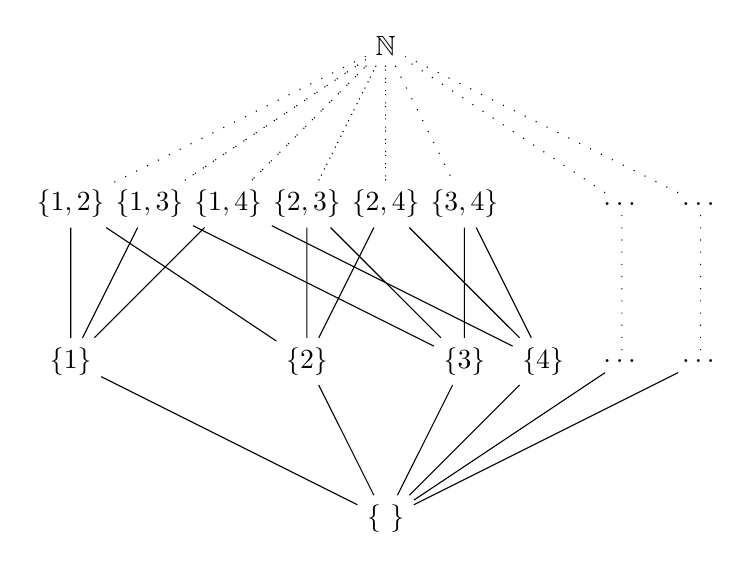
\begin{tikzpicture} % should make python program :(
  \node (one_s) at (1,4) {$\mathbb{N}$};
  \node (one) at (-3,0) {$\{1\}$};
  \node (two) at (0,0) {$\{2\}$};
  \node (three) at (2,0) {$\{3\}$};
  \node (four) at (3,0) {$\{4\}$};
  \node (rest_single) at (4,0) {$\dots$};
  \node (rest_single_2) at (5,0) {$\dots$};
  \node (rest_pair) at (4,2) {$\dots$};
  \node (rest_pair_2) at (5,2) {$\dots$};
  
  \node (one_two) at (-3,2) {$\{1,2\}$};
  \node (one_three) at (-2,2) {$\{1,3\}$};
  \node (one_four) at(-1,2) {$\{1,4\}$};
  \node (two_three) at (0,2) {$\{2,3\}$};
  \node (two_four) at (1,2) {$\{2,4\}$};
  \node (three_four) at (2,2) {$\{3,4\}$};
  
  \node (zero) at (1,-2) {$\{ \ \}$};
  
  \draw (zero) -- (one) -- (one_two) -- (two);
  \draw (zero) -- (two) -- (two_three) -- (three);
  \draw (zero) -- (three) -- (three_four) -- (four) -- (zero);
  \draw (zero) -- (rest_single);
  \draw (zero) -- (rest_single_2);	
	
  
  \draw (one) -- (one_three);
  \draw (one) -- (one_four);
  \draw (two) -- (two_four);
  \draw (three) -- (one_three);
  \draw (four) -- (one_four);
  \draw (four) -- (two_four);  
  

  \draw[loosely dotted] (one_two) -- (one_s) -- (one_three) -- (one_s) -- (one_four) -- (one_s) -- (two_three) -- (one_s) -- (two_four) -- (one_s) -- (three_four);

  \draw[loosely dotted] (rest_single) -- (rest_pair) -- (one_s);
  \draw[loosely dotted] (rest_single_2) -- (rest_pair_2) -- (one_s);
  
\end{tikzpicture}
\end{figure}
\end{frame}

\begin{frame}
\frametitle{Naravna števila za deljivost}
\begin{center}
$\mathbb{N}, |$
\end{center}
\begin{figure}
\centering
\begin{tikzpicture} % should make python program :(
  \node (one) at (1,4) {$0$};
  \node (two) at (-3,0) {$2$};
  \node (three) at (-1,0) {$3$};
  \node (five) at (2,0) {$5$};
  \node (rest_primes) at (4,0) {$\dots$};
  \node (rest_primes_2) at (5,0) {$\dots$};
  \node (rest_second) at (4,2) {$\dots$};
  \node (rest_second_2) at (5,2) {$\dots$};
  
  \node (four) at (-3,2) {$4$};
  \node (six) at (-2,2) {$6$};
  \node (nine) at (-1,2) {$9$};
  \node (ten) at (0,2) {$10$};
  \node (fifteen) at (1, 2) {$15$};
  \node (twentyfive) at (2,2) {$25$};
  
  \node (zero) at (1,-2) {$1$};
  
  \draw (zero) -- (two) -- (six) -- (three) -- (fifteen) -- (five) -- (zero) -- (rest_primes);
  \draw (rest_primes_2) -- (zero) -- (three);


  \draw (two) -- (four);
  \draw (three) -- (nine);
  \draw (two) -- (ten) -- (five);
  \draw (five) -- (twentyfive);
  \draw[loosely dotted] (four) -- (one);  
  \draw[loosely dotted] (six) -- (one);  
  \draw[loosely dotted] (nine) -- (one);  
  \draw[loosely dotted] (ten) -- (one);
  \draw[loosely dotted] (fifteen) -- (one);  
  \draw[loosely dotted] (twentyfive) -- (one);  
  \draw[loosely dotted] (rest_primes) -- (rest_second) -- (one);
  \draw[loosely dotted] (rest_primes_2) -- (rest_second_2) -- (one);
  
\end{tikzpicture}
\end{figure}
\end{frame}


\begin{frame}
\frametitle{Polne mreže}
\begin{definition}
Mreža $\mathcal{L}$ je polna, če za poljubno $\mathcal{A} \subseteq \mathcal{L}$ obstajata infimum in supremum za $\mathcal{A}$.
\end{definition}

\begin{example}
Poljubna linearna omejena mreža je polna, na nasproten način pa dobimo mreže, ki niso polne: $\mathbb{R}, \leq$.
\end{example}

\end{frame}

\begin{frame}
\frametitle{Zakoni v mrežah}
\begin{block}{Zakoni v mrežah}
\begin{itemize}
\item $x \lor x = x$, $x \land x = x$ (Idempotentnost)
\item $x \lor y = y \lor x$, $x \land y = y \land x$ (Komutativnost)
\item $(x \lor y) \lor z = x \lor (y \lor z)$\\ $(x \land y) \land z = x \land (y \land z)$ (Asociativnost)
\item $ x \lor (x \land y) = x$\\ $x \land (x \lor y) = x$ (Absorbcija)
\end{itemize}
\end{block}
\end{frame}


\begin{frame}
\frametitle{Asociativnost}
\begin{proof}
$$a = (x \lor y) \lor z, \ \ b = x \lor (y \lor z)$$ 
$$a \geq z, a \geq (x \lor y) \implies a \geq x, a \geq y$$\pause 
$$a \geq (y \lor z), a \geq x \lor (y \lor z) \implies a \geq b $$ \\ 
\centering Podobno v drugo smer, zaradi antisimetričnosti
$$ a = b$$

\end{proof}

%\begin{proof}
%Naj bo $a = (x \lor y) \lor z$ in $b = x \lor (y \lor z)$ \\ \pause
%Iz definicje ali sledi $a \geq z$ in $a \geq (x \lor y)$ in torej $a \geq x, a \geq y$ \\ \pause
%Potem velja tudi $a \geq (y \lor z)$ in $a \geq x \lor (y \lor z)$ torej $a \geq b$\\ \pause
%Na skoraj enak naredimo iz druge strani in dobimo $b \geq a$, ker pa je zaradi antisimetričnosti %relacije mogoče zgolj, kadar velja $a=b$
%\end{proof}
\end{frame}

\begin{frame}
\frametitle{Absorbcija}

%\begin{proof}
%Iz definicije ali vemo $x \leq (x \lor y)$ in $x \leq x$ torej $x \leq x \land (x \lor y)$\\ \pause
%Iz definicije in pa sledi $x \geq x \land (x \lor y)$\\ \pause
%Torej $x \leq x \land (x \lor y)$ in $x \geq x \land (x \lor y)$, dobimo $x = x \land (x \lor y)$
%\end{proof}

\begin{proof}
$$ x \leq (x \lor y), \ x \leq x \implies x \leq x \land (x \lor y)$$
$$x \geq x \land (x \lor y)$$
$$x \leq x \land (x \lor y), x \geq x \land (x \lor y)$$ \pause
$$x = x \land (x \lor y)$$
\end{proof}

\end{frame}


\begin{frame}
\begin{theorem}
Če imamo množico $\mathcal{L}$, za katero sta definirani operaciji $\lor, \land$ in če za te dve operacji veljajo zgornji zakoni, potem je ta množica mreža.
\end{theorem}
\end{frame}

\begin{frame}

\begin{block}{Dokaz}
\centering Definiramo: $x \leq y \iff x \land y = x$ \\ Preverimo, da je to delna urejenost \\ \pause 
Refleksivnost: $x \land x = x \implies x \leq x$\\ \pause
Antisimetričnost: $x \leq y, \ y \leq x \implies x \land y = x, y \land x = y$, uporabimo komutativnost in dobimo $x = y$\\ \pause
Tranzitivnost:  $x \leq y, y \leq z \implies x = x \land y, y = y \land z$ \\
$x = x \land (y \land z) = (x \land y) \land z = x \land z \implies x \leq z$ \\ \pause
Preverimo še, da velja $x \land y = x \iff x \lor y = y$\\ \pause
Uporabimo zadnji zakon in $x \lor y = (x \lor y) \land y = b$ in identično v drugo smer.
\end{block}

%\begin{block}{Dokaz}
%Najprej definiramo relacijo, naj za $x,y \in \mathcal{L}$ velja $x \leq y \iff x \land y = x$\\ in preverimo, da je to delna urejenost \\ \pause
%Refleksivnost: \pause$x \land x = x$ torej $x \leq x$\\ \pause
%Antisimetričnost: \pause $x \leq y$ in $y \leq x$, torej $x \land y = x$ in $y \land x = y$, uporabimo komutativnost in dobimo $x = y$\\ \pause
%Tranzitivnost: \pause $x \leq y$ in $y \leq z$ torej velja $x = x \land y$ in $y = y \land z$ \\ \pause
%Namesto $y$ uporabimo $y \land z$ in dobimo $x = x \land (y \land z) = (x \land y) \land z = x \land z$ torej \pause $x \leq z$ \\ \pause
%Preverimo še, da velja $x \land y = x \iff x \lor y = y$\\ \pause
%Uporabimo zadnji zakon in $x \lor y = (x \lor y) \land y = b$ in identično v drugo smer.
%\end{block}

\end{frame}


\begin{frame}
\begin{proof}
\centering
Poglejmo si zgolj supremum\\ \pause
Ponuja se $x \lor y$, ki je očitno zgornja meja
\begin{center}
$z \geq x, z \geq y \implies x \lor z = y \lor z = z$ \pause
\end{center} 
$$(x \lor y) \lor z = x \lor (y \lor z) = x \lor z = z \implies x \lor y \leq z$$
\end{proof}

%\begin{proof}
%Preveriti moramo še infimume in supremume\pause, poglejmo si samo supremum\\ \pause
%Sama od sebe se nam kot zgornja meja $x$ in $y$ ponuja $x \lor y$, ki je očitno zgornja meja \\ \pause%ker smo obstoj relacije že dokazali, lahko sedaj uporabljamo vse kar nam de
%Naj bo $z$ neka zgornja meja $x,y$, $x \lor z = y \lor z = z$\\ \pause
%Dobimo $(x \lor y) \lor z = x \lor (y \lor z) = x \lor z = z$, kar pomeni, da $x \lor y \leq z$, torej je $x \lor y$ natančna zgornja meja. 
%\end{proof}

\end{frame}

\begin{frame}

\begin{block}{}
Naravno se pojavi vprašanje, ali za operaciji v mrežah obstaja kakšne vrste enota ali celo inverz.
\end{block}

\begin{definition}
Če v mreži obstaja največji element, potem ta element označimo z $1$ ($\forall x \in \mathcal{L}. \ x \leq 1$)
\end{definition}

\begin{definition}
Če v mreži obstaja najmanjši element, potem ta element označimo z $0$ ($\forall x \in \mathcal{L}. \ x \geq 0$)
\end{definition}

\end{frame}

\begin{frame}
\begin{block}{}
Če v mreži obstajata $0$ in $1$ potem velja:
\begin{itemize}
\item $x \lor 1 = 1$
\item $x \lor 0 = x$
\item $x \land 0 = 0$
\item $x \land 1 = x$
\end{itemize}
\end{block}

\pause
\begin{example}
$0$ za $\mathbb{N}, |$\\ $\{ \}, \mathbb{N}$ za $\mathcal{P}(\mathbb{N})$
\end{example}

\end{frame}

\begin{frame}
\begin{definition}
V mreži z elementoma $0$ in $1$ elementa $x$ in $x'$ imenujemo \textbf{komplementarna}, če velja:
\begin{itemize}
\item $x \lor x' = 1$
\item $x \land x' = 0$
\end{itemize}
\end{definition}

\begin{definition}
Mrežo, v katri poljubnemu $x$ pripada \textbf{vsaj} en komplement imenujemo \textbf{komplementarna mreža}.
\end{definition}

\end{frame}

\begin{frame}
\begin{example}
Tipičen primer so vektorski podprostori nekega prostora $\mathcal{V}$, $1$ je celoten podprostor, $0$ je ničelni podprostor, komplementi poasmeznih elementov pa so kar ortogonalni komplementi.
\end{example}

\begin{example}
Ravnina, premice na njej in točke\\
Komplementi premic so točke ki na njej ne ležijo, komplementi točk pa premice, ki ne vsebujejo teh točk.\\
Imamo lahko več komplementov.
\end{example}

\end{frame}

\begin{frame}
\begin{definition}
Neprazna množica $\mathcal{M} \subseteq \mathcal{L}$ je \textbf{podmreža}, če je tudi sama mreža za isti operaciji in se na njih ujema. Povedano drugače $x \lor y \in \mathcal{M}$ in $x \land y \in \mathcal{M}$
\end{definition}
\end{frame}

\begin{frame}
\begin{theorem}
Če v mreži $\mathcal{L}$ vzamemo poljubna $x \leq y$, potem je množica $\mathcal{L}(x,y) := \{ z \in \mathcal{L} | \ x \leq z \leq y \}$ podmreža mreže $\mathcal{L}$.
\end{theorem}

\begin{proof}
Preprosto preverimo obstoj imfimuma in supremuma\\ \pause
Vzemimo poljubna $x',y' \in \mathcal{L}(x,y)$ in preverimo zaprtost\\ \pause $x \geq x' \lor y' \geq x' \land y' \geq y$
\end{proof}

\end{frame}


\begin{frame}
\frametitle{$\mathcal{P}(\{1,2,3,4\}), \subseteq$}
\begin{figure}
\centering
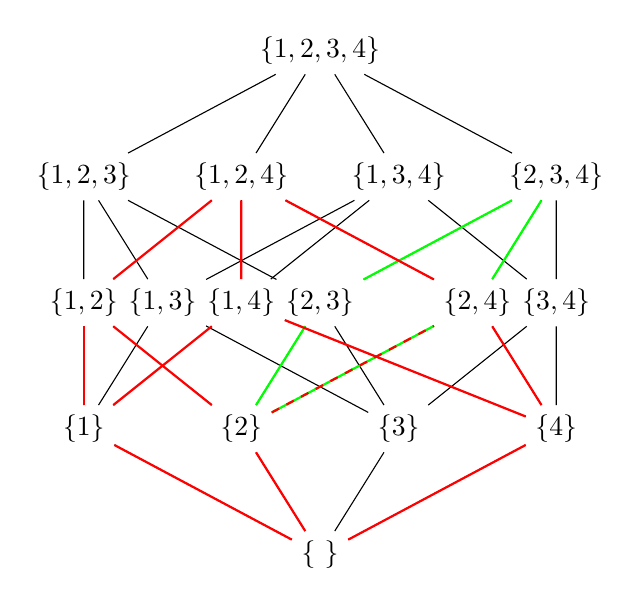
\begin{tikzpicture}[yscale=0.8] % should make python program :(
  \node (one_s) at (0,6) {$\{1,2,3,4\}$};
  \node (one) at (-3,0) {$\{1\}$};
  \node (two) at (-1,0) {$\{2\}$};
  \node (three) at (1,0) {$\{3\}$};
  \node (four) at (3,0) {$\{4\}$};
  
  \node (one_two) at (-3,2) {$\{1,2\}$};
  \node (one_three) at (-2,2) {$\{1,3\}$};
  \node (one_four) at(-1,2) {$\{1,4\}$};
  \node (two_three) at (0,2) {$\{2,3\}$};
  \node (two_four) at (2,2) {$\{2,4\}$};
  \node (three_four) at (3,2) {$\{3,4\}$};
  
  \node (four_m) at (-3,4) {$\{1,2,3\}$};

  \node (three_m) at (-1,4) {$\{1,2,4\}$};
  \node (two_m) at (1,4) {$\{1,3,4\}$};
  \node (one_m) at (3,4) {$\{2,3,4\}$};
      
  \node (zero) at (0,-2) {$\{ \ \}$};
  
  \draw (zero) -- (one) -- (one_two) -- (four_m) -- (one_s) -- (two_m) -- (one_three);
  \draw (zero) -- (two) -- (two_three) -- (three);
  \draw (zero) -- (three) -- (three_four) -- (four) -- (zero);
  \draw (one_two) -- (three_m) -- (one_s) -- (one_m) -- (three_four);
  \draw (one_three) -- (four_m) -- (two_three) -- (one_m) -- (two_four) -- (three_m);
  \draw (one_four) -- (three_m);
  \draw (one_four) -- (two_m) -- (three_four);
  
  \draw (one) -- (one_three);
  \draw (one) -- (one_four);
  \draw (two_four)--(two) -- (one_two);
  \draw (three) -- (one_three);
  \draw (four) -- (one_four);
  \draw (four) -- (two_four);  
  
  \draw[green, thick](two)--(two_three) -- (one_m) -- (two_four) -- (two);

  \draw[red, thick](zero)-- (one) -- (one_four);
  \draw[red, thick](three_m) -- (two_four) -- (four) -- (zero) -- (two) -- (one_two) -- (three_m) -- (one_four) -- (four);
  \draw[red, thick] (one) --(one_two);
  \draw[red, thick, dashed] (two) --(two_four);
  
\end{tikzpicture}
\end{figure}
\end{frame}


\begin{frame}
\begin{columns}
\begin{column}{5cm}
\begin{center}
$\{0,1\}, \subseteq$
\end{center}
\begin{figure}
\centering
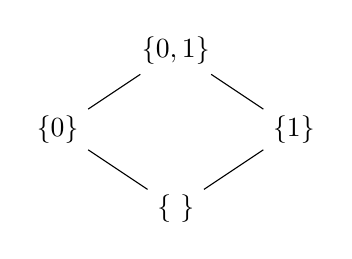
\begin{tikzpicture}[scale=0.5]
  \node (one) at (0,2) {$\{0,1\}$};
  \node (a) at (-3,0) {$\{0\}$};
  \node (d) at (3,0) {$\{1\}$};
  \node (zero) at (0,-2) {$\{ \ \}$};
  \draw (zero) -- (a) -- (one)  -- (d) -- (zero);
\end{tikzpicture}
\end{figure}
\end{column}

\begin{column}{5cm}
\begin{center}
$\{1,2,3,6\}, |$
\end{center}
\begin{figure}
\centering
\begin{tikzpicture}[scale=0.5]
  \node (one) at (0,2) {$6$};
  \node (a) at (-3,0) {$2$};
  \node (d) at (3,0) {$3$};
  \node (zero) at (0,-2) {$1$};
  \draw (zero) -- (a) -- (one)  -- (d) -- (zero);
\end{tikzpicture}
\end{figure}
\end{column}
\end{columns}

\begin{block}{}
Mreži se zdita sumljivo podobni, ali lahko to kako posplošimo?
\end{block}

\end{frame}

\begin{frame}
\begin{definition}
Preslikava $f :\mathcal{L} \to \mathcal{L}'$ je \textbf{homomorfizem}, če za poljubna $x,y \in \mathcal{L}$ velja:
\begin{itemize}
\item $f(x \lor y) = f(x) \lor f(y)$
\item $f(x \land y) = f(x) \land f(y)$
\end{itemize}
\end{definition}

%% Tukej je treba povedati zakaj


\begin{block}{Funkcija za prej}
\begin{table}[]
\centering
\label{my-label}
\begin{tabular}{c|c}
x         & f(x) \\ \hline
$\{\}$    & $1$  \\
$\{0\}$   & $2$  \\
$\{1\}$   & $3$  \\
$\{1,2\}$ & $6$ 
\end{tabular}
\end{table}
\end{block}

\end{frame}

\begin{frame}
\begin{theorem}
Za nek homomorfizem $f$ velja $f(\mathcal{L})$ je podmreža $\mathcal{L}$.
\end{theorem}

\begin{remark}
Homomorfizem ohranja urejenost
\end{remark}
\end{frame}


\begin{frame}

\begin{theorem}
Bijektivna preslikava $f$, $f : \mathcal{L} \to \mathcal{L}'$ je izomorfizem, če ohranja red v obeh smereh
\end{theorem}

\begin{block}{Red se mora ohranjati v obeh smereh}
Identiteta : $(\mathbb{N}, |)  \to (\mathbb{N}, \leq) $
\end{block}
\end{frame}

\begin{frame}
\begin{definition}
Mreža je \textbf{distributivna}, če za $\lor$ in $\land$ veljata zakona:
\begin{itemize}
\item $(x \lor y) \land z = (x \land z) \lor (y \land z)$
\item $(x \land y) \lor z = (x \lor z) \land (y \lor z)$
\end{itemize}
\end{definition}


\begin{example}
Linearno urejena množica je distributivna.
Potenčna množica glede na inkluzijo je prav tako distributivna.
\end{example}

\end{frame}

\begin{frame}
\begin{theorem}
Če ima distributivna mreža $\mathcal{L}$ elementa $0,1$, potem ima vsak elementa največ en komplment (ni pa še zagotovljen obstoj komplementa)
\end{theorem}

\begin{proof}
Naj bo $a$ poljuben element mreže. Naj bosta $a'$ in $a''$ dva njegova komplementa.\\
$$ a'' = 1 \land a'' = (a \lor a') \land a'' = (a  \land a'') \lor (a' \land a'') =  a' \land a''. $$

Torej sledi $ a'' \leq a'$. Analogno pokažemo $a' \leq a''$ in sledi $ a' = a''.$

\end{proof}

\end{frame}

\begin{frame}
\begin{definition}
Distributivno mrežo v kateri ima vsak element komplement imenujemo \textbf{Boolova algebra}.
\end{definition}
\begin{example}
$\mathcal{P}(\mathbb{N}), \subseteq$, $\mathcal{A}' = \mathcal{A}^c$ 
\end{example}
\end{frame}

\begin{frame}
\begin{theorem}
V Boolovi algebri veljata pravili:
\begin{itemize}
\item $(x \lor y)' = x' \land y'$
\item $(x \land y)' = y' \lor x'$ 
\end{itemize}
\end{theorem}
\end{frame}

\begin{frame}
\begin{proof}
$$(x \land y) \lor (x' \lor y')$$  $$(x \lor x' \lor y') \land (y \lor x' \lor y')$$  $$(1 \lor y') \land (1 \lor x') = 1 \lor 1 = 1$$

$$(x \land y) \land (x' \lor y')$$  $$(x \land x' \land y') \lor (y \land x' \land y')$$  $$(0 \land y') \lor (0 \land x') = 0 \lor 0 = 0$$

\end{proof}

\end{frame}


\begin{frame}% pa pridimo do mreže brez urejenosti
\begin{definition}
Kolobar, v katerem je vsak element idempotenten imenujemo \textbf{Boolov kolobar}.
\end{definition}
\begin{example}
$\mathbb{Z}_2 \oplus \mathbb{Z}_2 \oplus \dots \oplus \mathbb{Z}_2$
\end{example}
\end{frame}


\begin{frame}
\begin{theorem}
Boolov kolobar ima karakteristiko $2$
\end{theorem}
\pause
\begin{proof}
$$(x + x) = (x + x)^2 = x^2 + x^2 + x^2 + x^2 = x + x = 2x$$ 
$$2x = 0 \implies x = -x$$
\end{proof}
\end{frame}

\begin{frame}


\begin{theorem}
Boolov kolobar je komutativen
\end{theorem}
\pause
\begin{proof}
$$(x + y) = (x+y)^2 = x^2 + xy + yx + y^2 = x + xy + yx + y$$ 
$$xy + yx = 0 \implies xy = -ba \implies xy = yx $$
\end{proof}
\end{frame}

\begin{frame}
\begin{theorem}
Boolov kolobar je mreža za operaciji $x \lor y := x + y + xy$ in $x \land y := xy$
\end{theorem}
\end{frame}

\begin{frame}
\begin{proof}
Preverimo pravila
\begin{itemize}
\item $x \lor x = x + x + x^2 = 0 + x = x$, $x \land x = x^2 = x$
\item $x \lor y = x + y + xy = y + x + yx = y \lor x$, $x \land y = xy = yx = y \land y$\pause
\item $(x \lor y) \lor z  = x + y + z + xz + yz +xyz = x \lor (y \lor z)$\pause
$(x \land y) \land z = xyz = x \land (y \land z)$ 
\item $x \land (x \lor y) = x + xy + xy = x$\\ \pause
$x \lor (x \land y) = x + xy + xy = x$
\end{itemize}
\end{proof}
\end{frame}

\begin{frame}
\begin{theorem}
Boolov kolobar je distributivna mreža
\end{theorem}
\begin{proof}
$(x \lor y) \land z = xz + yz + xyz = (x \land z) \lor (y \land z)$ \\
$(x \land y) \lor z = xy + z + xyz = (x \lor z) \land (y \lor z)$
\end{proof}
\end{frame}

\begin{frame}
\begin{block}{}
$0$ je tudi $0$ za mrežo, $1$ prav tako(če obstaja)
\end{block}

\begin{block}{}
$x' = 1-x $ \\ \pause
$x \land (1-x) = x(1-x) = x - x = 0 $
$x \lor x'= x + (1-x) + x(1-x) = 1 $
\end{block}


\end{frame}

\begin{frame}
\begin{block}
V kolikor ima boolov kolobar enoto, potem je booova algebra (komplementarna distributivna mreža)
Velja pa tudi obratno, v komplementarni distributivni mreži lahko definiramo z $\lor, \land$ definiramo seštevanje in množenje kot notranji operaciji.
\end{block}
\end{frame}

\begin{frame}
\frametitle{Boolov kolobar}
\begin{center}
$\mathbb{Z}_2 \oplus \mathbb{Z}_2 \oplus \mathbb{Z}_2$
\end{center}
\begin{figure}
\centering
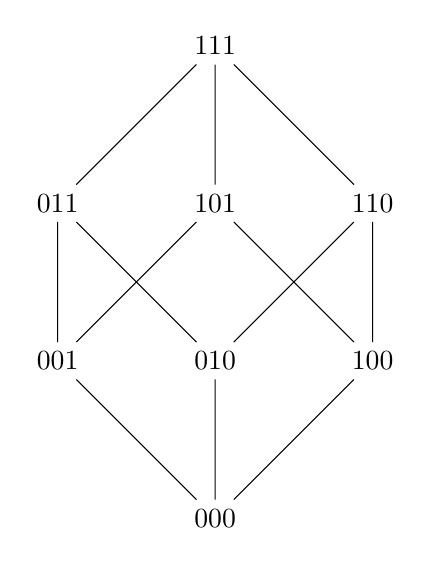
\begin{tikzpicture} % should make python program :(
  \node (one) at (0,0) {$111 $};
  \node (two) at (-2,-4) {$001 $};
  \node (three) at (0,-4) {$010 $};
  \node (five) at (2,-4) {$100 $};
  
  \node (four) at (-2,-2) {$011 $};
  \node (six) at (0,-2) {$101 $};
  \node (nine) at (2,-2) {$110 $};
  
  \node (zero) at (0,-6) {$000 $};
  
  \draw (zero) -- (two) -- (four) -- (one) -- (six) -- (two);  
  \draw (zero) -- (three) -- (four);
  \draw (zero) -- (five) -- (six);
  \draw (three) -- (nine);
  \draw (one) -- (nine) -- (five);
  
\end{tikzpicture}
\end{figure}
\end{frame}

\begin{frame}
\frametitle{Lastnosti boolovih kolobarjev}
\begin{block}{}
\begin{itemize}
\item Boolove mreže imajo $2^n$ elementov za nek $n \in \mathbb{N}$
\item Za poljubno naravno število $n$ je mreža vseh deljiteljev tega števila boolova mreža natanko tedaj, ko $n$ ni deljiv s kvadratom kakega naravnega števila\\
\item Mreža $n$ kopij $\mathbb{Z}_2$ je graf $n-$kocke
\item Elementi v boolovi mreži so direktno povezani z elementi, ki so od njih \textit{oddaljeni} za največ $1$
\item Boolovi mreži sta si izomorfni, če imata enako število elementov
\item Deljitelji $30$ urejeni po deljivosti so boolova mreža, ki je izomorfna $\mathbb{Z}_2 \oplus \mathbb{Z}_2 \oplus \mathbb{Z}_2$
\end{itemize}

\end{block}
\end{frame}

\begin{frame}
\frametitle{Boolove mreže}
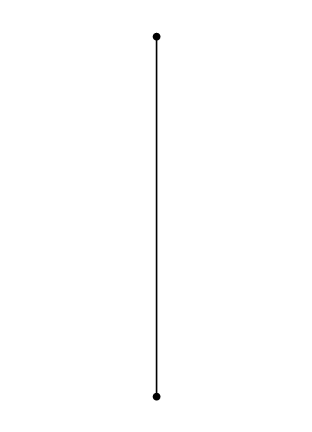
\includegraphics[scale=0.2]{bool1}
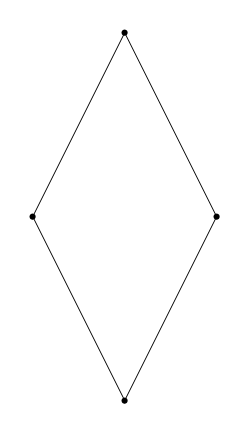
\includegraphics[scale=0.2]{bool2}
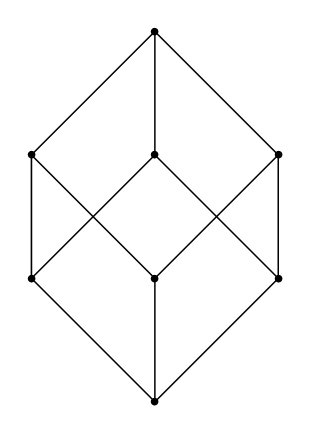
\includegraphics[scale=0.2]{bool3}
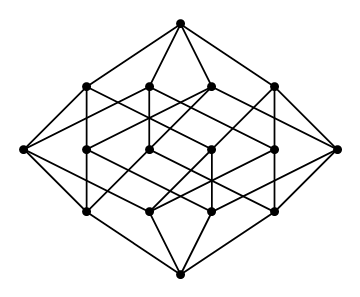
\includegraphics[scale=0.29]{bool4}
\end{frame}


%\begin{frame} Bom to omenil jaz.
%\begin{definition}
%Komplementarno in distributivno mrežo imenujemo \textbf{Boolova algebra}.
%\end{definition}

%\begin{block}{}
%To ni algebra?????
%\end{block}
%\end{frame}

\begin{frame}
\section{Modulske mreže}
\begin{definition}
Mreža $\mathcal{L}$ je \textbf{modulska} mreža, če za $a \leq c$ velja:
$$(a \lor b) \land c = a \lor (b \land c)$$
\end{definition}
\end{frame}


\begin{frame}
\begin{block}{}
Primer: $\mathcal{G}$ grupa in označimo z $\mathcal{L}$ množico vseh  njenih podgrup edink. Množico $\mathcal{L}$ uredimo glede na inkluzijo. Naj bosta $\mathcal{H}$  in $\mathcal{K}$ dve podgrupi edinki $\mathcal{G}$. Za infinum dveh podrup vzamemo presek, za supremum pa izberemo produkt $\mathcal{HK}$.
\end{block}
\end{frame}

\begin{frame}
\begin{theorem}
Mreža podgrup edink je modulska.
\end{theorem}
\end{frame}

\begin{frame}
\begin{block}{Dokaz:}
Naj bo $\mathcal{G}$ grupa in $\mathcal{H}$, $\mathcal{K}$ in $\mathcal{L}$ njene podgrupe edinke in naj velja $\mathcal{H} \leq \mathcal{L}$. Vemo, da $\mathcal{H} \lor \mathcal{K} =\mathcal{H}\mathcal{K}.$\\
Poglejmo si ($\mathcal{H} \lor \mathcal{K}) \land \mathcal{L}$.
\end{block}
\end{frame}

\begin{frame}
\begin{definition}
Elementa $a$, $b$ sta soseda, če velja: $a$ $\leq$ $b$ in če iz $a$ $\leq$ $c$ in $c$ $\leq$ $b$ sledi $c = a$ ali $c = b$.
Zaporedje elementov $a, b, c, ..., x$ bomo imenovali \textbf{veriga}, če sta vsaka dva zaporedna elementa soseda in velja $a \leq b, b \leq c, ...$. Ta veriga veže elementa $a in x.$
\end{definition}
\begin{block}{}
Dva elementa mreže je možno povezati z več različnimi verigami.
\end{block}
\end{frame}

\begin{frame}
\begin{block}{}
Brez dokaza navedimo naslednji izrek:
\end{block}
\begin{theorem}
Vse verige, ki v modulski mreži vežejo isti par elementov, so enako dolge.
\end{theorem}
\begin{block}{}
Ideja o definiranju dimenzije mreže.
\end{block}
\end{frame}

\end{document}
